% В тексте следует применять научно-технические термины, обозначения
% и определения, установленные действующими стандартами, а при их
% отсутствии – принятые в научно-технической литературе.
% Запрещается применять иностранные термины при наличии
% равнозначных слов и терминов в русском языке.

% cargo make run_mock_robot
% cargo make brains
% cargo make gui


% https://tex.stackexchange.com/questions/498098/how-to-fix-xelatex-warnings-about-undefined-font-shapes
% !TeX spellcheck = russian-aot-ieyo

% Зачем: Определяет класс документа (То, как будет выглядеть документ)
% Примечание: параметр draft помечает строки, вышедшие за границы страницы, прямоугольником, в финальной версии его нужно удалить.
% \documentclass[a4paper,14pt,russian,oneside,final,draft]{extreport}
\documentclass[a4paper,14pt,russian,oneside,final]{extreport}
\usepackage{cite}
\usepackage{float}
%\restylefloat{table}

% Rust programming language

% Зачем: Учет особенностей различных языков.
\usepackage[english,russian]{babel}

% Зачем: что-то чтобы док получился лучше, используем новую кодировку для всяких символов
\usepackage[T2A]{fontenc} 
% Set TimeNewRoman as main font
\usepackage{fontspec}
\setmainfont{Times New Roman}
\setmonofont{Consolas}


%\input{fonts_linux}% не забудьте закомментировать \input{fonts_windows}

% Зачем: Установка кодировки исходных файлов.
% UPD: не надо если использовать изначально движок который делает
% \usepackage[utf8]{inputenc}

% Зачем: Делает результирующий PDF "searchable and copyable".
\usepackage{cmap}

% Зачем: Чтобы можно было использовать русские буквы в формулах, но в случае использования предупреждать об этом.
\usepackage[warn]{mathtext}


% Зачем: Добавляет поддержу дополнительных размеров текста 8pt, 9pt, 10pt, 11pt, 12pt, 14pt, 17pt, and 20pt.
% Почему: Пункт 2.1.1 Требований по оформлению пояснительной записки.
\usepackage{extsizes}


% Зачем: Длинна, пимерно соответвующая 5 символам
% Почему: Требования содержат странное требование про отсупы в 5 символов (для немоноширинного шрифта :| )
\newlength{\fivecharsapprox}
\setlength{\fivecharsapprox}{6ex}

\usepackage{placeins}


% Зачем: Добавляет отступы для абзацев.
% Почему: Пункт 2.1.3 Требований по оформлению пояснительной записки.
\usepackage{indentfirst}
\setlength{\parindent}{1.25cm} % 1.25 - 1.27 см абзацы


% Зачем: Настраивает отступы от границ страницы.
% Почему: Пункт 2.1.2 Требований по оформлению пояснительной записки.
\usepackage[left=3cm,top=2.0cm,right=1.5cm,bottom=2.7cm,footskip=1.3cm]{geometry}
\usepackage{microtype}


% Зачем: Настраивает межстрочный интервал, для размещения 40 +/- 3 строки текста на странице.
% Почему: Пункт 2.1.1 Требований по оформлению пояснительной записки.
\usepackage[nodisplayskipstretch]{setspace} 
\setstretch{1.0}

% Зачем: Отключает использование изменяемых межсловных пробелов.
% Почему: Так не принято делать в текстах на русском языке.
\frenchspacing

% Зачем: Сброс счетчика сносок для каждой страницы
% Примечание: в "Требованиях по оформлению пояснительной записки" не указано,
% как нужно делать, но в других БГУИРовских докуметах рекомендуется нумерация
% отдельная для каждой страницы
\usepackage{perpage}
\MakePerPage{footnote}




% Зачем: Добавляет скобку 1) к номеру сноски
% Почему: Пункты 2.9.2 и 2.9.1 Требований по оформлению пояснительной записки.
\makeatletter 
\def\@makefnmark{\hbox{\@textsuperscript{\normalfont\@thefnmark)}}}
\makeatother


% Зачем: Расположение сносок внизу страницы
% Почему: Пункт 2.9.2 Требований по оформлению пояснительной записки.
\usepackage[flushmargin, bottom]{footmisc}
\setlength{\footnotemargin}{\fivecharsapprox}

% Зачем: Переопределяем стандартную нумерацию, т.к. в отчете будут только section и т.д. в терминологии TeX
\makeatletter
\renewcommand{\thesection}{\arabic{section}}
\makeatother


% Зачем: Пункты (в терминологии требований) в терминологии TeX subsubsection должны нумероваться
% Почему: Пункт 2.2.3 Требований по оформлению пояснительной записки.
\setcounter{secnumdepth}{3}


% Зачем: Настраивает отступ между таблицей с содержанимем и словом СОДЕРЖАНИЕ
% Почему: Пункт 2.2.7 Требований по оформлению пояснительной записки.
\usepackage{tocloft}
\setlength{\cftbeforetoctitleskip}{-1em}
\setlength{\cftaftertoctitleskip}{1em}
\renewcommand{\cfttoctitlefont}{\normalsize\bfseries}

% Зачем: Определяет отступы слева для записей в таблице содержания.
% Почему: Пункт 2.2.7 Требований по оформлению пояснительной записки.
\makeatletter
\renewcommand{\l@section}{\@dottedtocline{1}{0.5em}{1.2em}}
\renewcommand{\l@subsection}{\@dottedtocline{2}{1.7em}{2.0em}}
\makeatother


% Зачем: Работа с колонтитулами
\usepackage{fancyhdr} % пакет для установки колонтитулов

\pagestyle{fancy} % смена стиля оформления страниц


% Зачем: Нумерация страниц располагается справа снизу страницы
% Почему: Пункт 2.2.8 Требований по оформлению пояснительной записки.
\fancyhf{} % очистка текущих значений
\fancyfoot[R]{\thepage} % установка верхнего колонтитула
\renewcommand{\footrulewidth}{0pt} % убрать разделительную линию внизу страницы
\renewcommand{\headrulewidth}{0pt} % убрать разделительную линию вверху страницы
\fancypagestyle{plain}{ 
    \fancyhf{}
    \rfoot{\thepage}}


% Зачем: Задает стиль заголовков раздела жирным шрифтом, прописными буквами, без точки в конце
% Почему: Пункты 2.1.1, 2.2.5, 2.2.6 и ПРИЛОЖЕНИЕ Л Требований по оформлению пояснительной записки.
\makeatletter
\renewcommand\section{%
  \clearpage\@startsection {section}{1}%
    {\fivecharsapprox}%
    {-1em \@plus -1ex \@minus -.2ex}%
    {1em \@plus .2ex}%
    {\raggedright\hyphenpenalty=10000\normalfont\normalsize\bfseries\MakeUppercase}}
\makeatother


% Зачем: Задает стиль заголовков подразделов
% Почему: Пункты 2.1.1, 2.2.5 и ПРИЛОЖЕНИЕ Л Требований по оформлению пояснительной записки.
\makeatletter
\renewcommand\subsection{%
  \@startsection{subsection}{2}%
    {\fivecharsapprox}%
    {-1em \@plus -1ex \@minus -.2ex}%
    {1em \@plus .2ex}%
    {\raggedright\hyphenpenalty=10000\normalfont\normalsize\bfseries}}
\makeatother


% Зачем: Задает стиль заголовков пунктов
% Почему: Пункты 2.1.1, 2.2.5 и ПРИЛОЖЕНИЕ Л Требований по оформлению пояснительной записки.
\makeatletter
\renewcommand\subsubsection{
  \@startsection{subsubsection}{3}%
    {\fivecharsapprox}%
    {-1em \@plus -1ex \@minus -.2ex}%
    {\z@}%
    {\raggedright\hyphenpenalty=10000\normalfont\normalsize\bfseries}}
\makeatother

% Зачем: для оформления введения и заключения, они должны быть выровнены по центру.
% Почему: Пункты 1.1.15 и 1.1.11 Требований по оформлению пояснительной записки.
\makeatletter
\newcommand\sectioncentered{%
  \clearpage\@startsection {section}{1}%
    {\z@}%
    {-1em \@plus -1ex \@minus -.2ex}%
    {1em \@plus .2ex}%
    {\centering\hyphenpenalty=10000\normalfont\normalsize\bfseries\MakeUppercase}%
    }
\makeatother



% Зачем: Задает стиль библиографии
% Почему: Пункт 2.8.6 Требований по оформлению пояснительной записки.
\usepackage[square,numbers,sort&compress]{natbib}
\usepackage{usebib}
% \bibliographystyle{styles/belarus-specific-utf8gost780u}
\bibliographystyle{belarus-specific-utf8gost780u}


% Зачем: Пакет для вставки картинок
% Примечание: Объяснение, зачем final - http://tex.stackexchange.com/questions/11004/why-does-the-image-not-appear
\usepackage[final]{graphicx}
\DeclareGraphicsExtensions{.pdf,.png,.jpg,.eps}



% Зачем: Директория в которой будет происходить поиск картинок
\graphicspath{{./images/}}


% Зачем: Добавление подписей к рисункам
\usepackage[nooneline]{caption}
\usepackage{subcaption}
\usepackage[skip=0pt]{caption}



% Зачем: чтобы работала \No в новых латехах
\DeclareRobustCommand{\No}{\ifmmode{\nfss@text{\textnumero}}\else\textnumero\fi}

% Зачем: поворот ячеек таблиц на 90 градусов
\usepackage{rotating}
\DeclareRobustCommand{\rotatedtext}[1]{\begin{sideways}{#1}\end{sideways}}


% Зачем: когда в формулах много кириллических символов команда \text{} занимает много места
\DeclareRobustCommand{\x}[1]{\text{#1}}


% Зачем: Задание подписей, разделителя и нумерации частей рисунков
% Почему: Пункт 2.5.5 Требований по оформлению пояснительной записки.
\DeclareCaptionLabelFormat{stbfigure}{Рисунок #2}
\DeclareCaptionLabelFormat{stbtable}{Таблица #2}
\DeclareCaptionLabelSeparator{stb}{~--~}
\captionsetup{labelsep=stb}
\captionsetup[figure]{labelformat=stbfigure,justification=centering}
\captionsetup[table]{labelformat=stbtable,justification=raggedright,skip=0pt}
\renewcommand{\thesubfigure}{\asbuk{subfigure}}

% Зачем: Окружения для оформления формул
% Почему: Пункт 2.4.7 требований по оформлению пояснительной записки и специфические требования различных кафедр
% Пример использования смотри в course_content.tex, строка 5
\usepackage{calc}
\newlength{\lengthWordWhere}
\settowidth{\lengthWordWhere}{где}

\newenvironment{explanationx}
    {%
    %%% Define the itemize environment with specific parameters
    \begin{itemize}[%
		leftmargin=0cm,
        %leftmargin=0cm, % No left margin for the entire list
        itemindent=\parindent, % Indent the item label by \parindent
        labelsep=\labelsep, % Space between label and item content
        labelwidth=0cm] % Width of the label (assumed to be defined elsewhere)
    \renewcommand\labelitemi{}% Remove the bullet for items
    }
    {%
    \end{itemize}
    }

% \newenvironment{explanationx}
%     {%
%     %%% Следующие строки определяют специфические требования разных редакций стандартов. Раскоменнтируйте нужную строку
%     %% стандартный абзац, СТП-01 2010
%     %\begin{itemize}[leftmargin=0cm, itemindent=\parindent + \lengthWordWhere + \labelsep, labelsep=\labelsep]
%     %% без отступа, СТП-01 2013
%     %\begin{itemize}[leftmargin=0cm, itemindent=\lengthWordWhere + \labelsep , labelsep=\labelsep]%
%     \renewcommand\labelitemi{}%
%     }
%     {%
%     %\\[\parsep]
%     \end{itemize}
%     }

% Старое окружение для "где". Сохранено для совместимости
\usepackage{tabularx}

\newenvironment{explanation}
    {
    %%% Следующие строки определяют специфические требования разных редакций стандартов. Раскоменнтируйте нужные 2 строки
    %% стандартный абзац, СТП-01 2010
    %\par 
    %\tabularx{\textwidth-\fivecharsapprox}{@{}ll@{ --- } X }
    %% без отступа, СТП-01 2013
    \noindent 
    \tabularx{\textwidth}{@{}ll@{ --- } X }
    }
    { 
    \\[\parsep]
    \endtabularx
    }


% Зачем: Удобная вёрстка многострочных формул, масштабирующийся текст в формулах, формулы в рамках и др
\usepackage{amsmath}


% Зачем: Поддержка ажурного и готического шрифтов 
\usepackage{amsfonts}


% Зачем: amsfonts + несколько сотен дополнительных математических символов
\usepackage{amssymb}


% Зачем: Окружения «теорема», «лемма»
\usepackage{amsthm}


% Зачем: Производить арифметические операции во время компиляции TeX файла
\usepackage{calc}

% Зачем: Производить арифметические операции во время компиляции TeX файла
\usepackage{xfp}
\usepackage{fp}

% Зачем: Пакет для работы с перечислениями
\usepackage{enumitem}
\makeatletter
 \AddEnumerateCounter{\asbuk}{\@asbuk}{щ)}
\makeatother


% Зачем: Устанавливает символ начала простого перечисления
% Почему: Пункт 2.3.5 Требований по оформлению пояснительной записки.
\setlist{nolistsep}


% Зачем: Устанавливает символ начала именованного перечисления
% Почему: Пункт 2.3.8 Требований по оформлению пояснительной записки.
\renewcommand{\labelenumi}{\asbuk{enumi})}
\renewcommand{\labelenumii}{\arabic{enumii})}

% Зачем: Устанавливает отступ от границы документа до символа списка, чтобы этот отступ равнялся отступу параграфа
% Почему: Пункт 2.3.5 Требований по оформлению пояснительной записки.

\setlist[itemize,0]{itemindent=\parindent + 2.2ex, leftmargin=0ex, label=--, labelwidth=2em, rightmargin=0pt, listparindent=\parindent}
\setlist[enumerate,1]{itemindent=\parindent + 2.7ex, leftmargin=0ex, rightmargin=0pt, listparindent=\parindent}
\setlist[enumerate,2]{itemindent=\parindent + \parindent - 2.7ex, rightmargin=0pt, listparindent=\parindent}

%\setlist[itemize,0]{itemindent=\parindent + 2.2ex, leftmargin=0ex, label=--, rightmargin=0pt, listparindent=\parindent}
%\setlist[enumerate,1]{itemindent=\parindent + 2.7ex, leftmargin=0ex, rightmargin=0pt, listparindent=\parindent}
%\setlist[enumerate,2]{itemindent=\parindent + \parindent - 2.7ex, rightmargin=0pt, listparindent=\parindent}

% Зачем: Включение номера раздела в номер формулы. Нумерация формул внутри раздела.
\AtBeginDocument{\numberwithin{equation}{section}}

% Зачем: Включение номера раздела в номер таблицы. Нумерация таблиц внутри раздела.
\AtBeginDocument{\numberwithin{table}{section}}

% Зачем: Включение номера раздела в номер рисунка. Нумерация рисунков внутри раздела.
\AtBeginDocument{\numberwithin{figure}{section}}


% Зачем: Дополнительные возможности в форматировании таблиц
\usepackage{makecell}
\usepackage{multirow}
\usepackage{array}


% Зачем: "Умная" запятая в математических формулах. В дробных числах не добавляет пробел
% Почему: В требованиях не нашел, но в русском языке для дробных чисел используется {,} а не {.}
\usepackage{icomma}

% Зачем: макрос для печати римских чисел
\makeatletter
\newcommand{\rmnum}[1]{\romannumeral #1}
\newcommand{\Rmnum}[1]{\expandafter\@slowromancap\romannumeral #1@}
\makeatother


% Зачем: Управление выводом чисел.
\usepackage{sistyle}
\SIdecimalsign{,}

% Зачем: inline-коментирование содержимого.
\newcommand{\ignore}[2]{\hspace{0in}#2}


% Зачем: Возможность коментировать большие участки документа
\usepackage{verbatim}


\usepackage{xcolor}


% Зачем: Оформление листингов кода
% Примечание: final нужен для переопределения режима draft, в котором листинги не выводятся в документ.
\usepackage[final]{listings}
\usepackage{listings-rust}

\newfontfamily\consolas{Consolas}
\lstset{
	% basicstyle=\small\consolas,
	basicstyle=\fontsize{12}{12}\consolas,
  breaklines=true,
  breakatwhitespace=true,
  breakindent=20pt, % or any value you prefer
  language=Rust,
  % ... other options ...
}

\makeatletter
\renewcommand{\@seccntformat}[1]{\csname the#1\endcsname\hspace{0.5em}} % Set space to 1em
\makeatother

\usepackage{titlesec}
\newcommand{\sectionbreak}{\clearpage}
\titleformat{\section}[block]
  {\raggedright\normalfont\bfseries} % format of the whole title
  {\raggedright\thesection}                % label (section number)
  {0.5em}                       % horizontal space between number and title
  {}

\titleformat{\subsection}[block]
  {\raggedright\normalfont\bfseries}
  {\raggedright\thesubsection}
  {0.5em}
  {}


\titleformat{\subsubsection}[block]
  {\raggedright\normalfont}
  {\raggedright\bfseries\thesubsubsection}
  {0.5em}
  {}

\titlespacing*{\section}{\parindent}{1em}{0.5em}
\titlespacing*{\subsection}{\parindent}{1em}{0.5em}
\titlespacing*{\subsubsection}{\parindent}{1em}{0.0em}

\usepackage{amsmath}

\usepackage{algorithm}
\usepackage{algpseudocode}


% Зачем: настройка оформления листинга для языка F#
\definecolor{bluekeywords}{rgb}{0.13,0.13,1}
\definecolor{greencomments}{rgb}{0,0.5,0}
\definecolor{turqusnumbers}{rgb}{0.17,0.57,0.69}
\definecolor{redstrings}{rgb}{0.5,0,0}

\renewcommand{\lstlistingname}{Листинг}

\lstdefinelanguage{FSharp}
    {morekeywords={abstract,and,as,assert,base,begin,class,default,delegate,do,done,downcast,downto,elif,else,end,exception,extern,false,finally,for,fun,function,global,if,in,inherit,inline,interface,internal,lazy,let,let!,match,member,module,mutable,namespace,new,not,null,of,open,or,override,private,public,rec,return,return!,select,static,struct,then,to,true,try,type,upcast,use,use!,val,void,when,while,with,yield,yield!,asr,land,lor,lsl,lsr,lxor,mod,sig,atomic,break,checked,component,const,constraint,constructor,continue,eager,event,external,fixed,functor,include,method,mixin,object,parallel,process,protected,pure,sealed,tailcall,trait,virtual,volatile},
    keywordstyle=\bfseries\color{bluekeywords},
    sensitive=false,
    morecomment=[l][\color{greencomments}]{///},
    morecomment=[l][\color{greencomments}]{//},
    morecomment=[s][\color{greencomments}]{{(*}{*)}},
    morestring=[b]",
    stringstyle=\color{redstrings},
    }

\lstdefinestyle{fsharpstyle}{
   xleftmargin=0ex,
   language=FSharp,
   basicstyle=\footnotesize\ttfamily,
   breaklines=true,
   columns=fullflexible
}

\lstdefinestyle{csharpinlinestyle} {
  language=[Sharp]C,
  morekeywords={yield,var,get,set,from,select,partial,where,async,await},
  breaklines=true,
  columns=fullflexible,
  basicstyle=\footnotesize\ttfamily
}

\lstdefinestyle{csharpstyle}{
  language=[Sharp]C,
  frame=lr,
  rulecolor=\color{blue!80!black}}


% Зачем: Нумерация листингов в пределах секции
\AtBeginDocument{\numberwithin{lstlisting}{section}}

\usepackage[normalem]{ulem}

\usepackage[final,hidelinks]{hyperref}
% Моноширинный шрифт выглядит визуально больше, чем пропорциональный шрифт, если их размеры одинаковы. Искусственно уменьшаем размер ссылок.
\renewcommand{\UrlFont}{\small\rmfamily\tt}

\setlength{\bibsep}{0em}

% Магия для подсчета разнообразных объектов в документе
\usepackage{lastpage}
\usepackage{totcount}
\regtotcounter{section}

\usepackage{etoolbox}

\newcounter{totfigures}
\newcounter{tottables}
\newcounter{totreferences}
\newcounter{totequation}

\providecommand\totfig{} 
\providecommand\tottab{}
\providecommand\totref{}
\providecommand\toteq{}

\makeatletter
\AtEndDocument{%
  \addtocounter{totfigures}{\value{figure}}%
  \addtocounter{tottables}{\value{table}}%
  \addtocounter{totequation}{\value{equation}}
  \immediate\write\@mainaux{%
    \string\gdef\string\totfig{\number\value{totfigures}}%
    \string\gdef\string\tottab{\number\value{tottables}}%
    \string\gdef\string\totref{\number\value{totreferences}}%
    \string\gdef\string\toteq{\number\value{totequation}}%
  }%
}
\makeatother

\pretocmd{\section}{\addtocounter{totfigures}{\value{figure}}\setcounter{figure}{0}}{}{}
\pretocmd{\section}{\addtocounter{tottables}{\value{table}}\setcounter{table}{0}}{}{}
\pretocmd{\section}{\addtocounter{totequation}{\value{equation}}\setcounter{equation}{0}}{}{}
\pretocmd{\bibitem}{\addtocounter{totreferences}{1}}{}{}



% Для оформления таблиц не влязящих на 1 страницу
\usepackage{longtable}

% Для включения pdf документов в результирующий файл
\usepackage{pdfpages}

% Для использования знака градуса и других знаков
% http://ctan.org/pkg/gensymb
\usepackage{gensymb}

% Зачем: преобразовывать текст в верхний регистр командой MakeTextUppercase
\usepackage{textcase}

% Зачем: чтобы выключать перенос слов (например в таблицах)
\usepackage{hyphenat}


% Зачем: Переносы в словах с тире.
% Тире в словае заменяем на \hyph: аппаратно\hyphпрограммный.
% https://stackoverflow.com/questions/2193307/how-to-get-latex-to-hyphenate-a-word-that-contains-a-dash#
\def\hyph{-\penalty0\hskip0pt\relax}

% Добавляем абзацный отступ для библиографии
% https://github.com/mstyura/bsuir-diploma-latex/issues/19
\setlength\bibindent{-1.0900cm}

\makeatletter
\renewcommand\NAT@bibsetnum[1]{\settowidth\labelwidth{\@biblabel{#1}}%
   \setlength{\leftmargin}{\bibindent}\addtolength{\leftmargin}{\dimexpr\labelwidth+\labelsep\relax}%
   \setlength{\itemindent}{-\bibindent+\fivecharsapprox-0.240cm}%
   \setlength{\listparindent}{\itemindent}
\setlength{\itemsep}{\bibsep}\setlength{\parsep}{\z@}%
   \ifNAT@openbib
     \addtolength{\leftmargin}{\bibindent}%
     \setlength{\itemindent}{-\bibindent}%
     \setlength{\listparindent}{\itemindent}%
     \setlength{\parsep}{10pt}%
   \fi
}


\begin{document}

\def \appname {ПСНМС}
\def \diplomaname {программное средство навигации мобильных систем}
\def \diplomanameR {программного средства навигации мобильных систем}
\def \ros {ROS}
\def \rosTwo {ROS2}

\newcommand{\todo}[1]{\textcolor{red}{TODO: #1}}
\newcommand{\review}[1]{\textcolor{green}{#1}}

\def \nr {\todo{need reference?}}

% Программное средство навигации мобильных систем
% Выбор языка должен быть в документе
\selectlanguage{russian}

\sectioncentered*{ОПРЕДЕЛЕНИЯ И СОКРАЩЕНИЯ}
В настоящей пояснительной записке применяются следующие определения и
сокращения.

\textit{Программное обеспечение} -- совокупность программ системы обработки
информации и программных документов, необходимых для эксплуатации этих
программ.

\textit{Планирование маршрута} - планирование маршрута относится к процессу
поиска оптимального пути между несколькими точками. Планирование маршрута обычно
характеризуется как проблема обхода графа, а алгоритмы, такие как A*, D* и RRT,
являются обычными вариантами для реализации.

\textit{Планирование движения} -- планирование движения относится к процессу
определения движения робота во времени, чтобы следовать определенной
траектории.

\textit{Фреймворк} -- программное обеспечение, облегчающее разработку и
объединение различных компонентов большого программного проекта.

\textit{Сериализация} -- процесс перевода структуры данных в битовую последовательность.

\textit{Десериализация} -- процесс создания структуры данных из битовой последовательности. .

DDS(Data distribution system) -- Служба распространения данных для систем
реального времени является стандартом межмашинного взаимодействия Object
Managment Group, целью которого является обеспечение масштабируемых,
оперативных, надежных, высокопроизводительных и совместимых обменов данными с
применением шаблона «издатель — подписчик»

SLAM(Simultaneous localization and mapping) -- одновременная локализация и
построение карты.

\ros -- Robot Operating System

\rosTwo{} - Robot Operating System 2

\renewcommand \contentsname {
	\centerline{\bfseries\large{\MakeUppercase{содержание}}}}
\newpage

{
% \normalsize\selectfont % Хак для уменьшения шрифта (у меня не работает)
\tableofcontents
\newpage
}

\sectioncentered*{ВВЕДЕНИЕ}
В современном мире развитие технологий автономных систем занимает одно из
ключевых мест в научно-техническом прогрессе. Автономная навигация мобильных
платформ представляет собой перспективное направление, которое находит
применение в различных областях: от робототехники и логистики до сельского
хозяйства.

Создание надежного и эффективного программного обеспечения для обеспечения
самостоятельного перемещения таких платформ является актуальной задачей.
требующей комплексного подхода к решению вопросов планирования маршрутов,
обработки данных с датчиков и адаптации к изменяющимся условиям окружающей
среды.

Задача автономной навигации мобильной системы концептуально звучит очень
просто -- система принимает данные с сенсоров и отправляет управляющие команды
на шасси. Для её реализации необходимо решить большое количество объёмных
задач: оценка текущей позиции, построение карты, построение машрута, получение
данных с сенсоров, обработка аварийных ситуаций, и т. д.

На данный момент стандартом индустрии является фреймворк для разработки
роботизированных систем \ros, который включает в себя фреймворк для навигации и
пакеты для решения задач связанных с навигацией (SLAM, локализация робота).
На основе данных фреймворков осуществ 

Целью данной работы является анализ существующих решений, а также
проектирование и разработка программного обеспечения, которое позволяет
осуществлять автономную навигацию мобильных платформ.

Разработка \diplomanameR{} позволяет создавать мобильные платформы с автономной
навигацией, что в свою очередь может быть применено для создания роботов для
перевозки грузов, роботов пылесосов, и других систем где требуется навигация
мобильной системы.

% BIG SECTION
\section{Аналитический обзор программных продуктов, литературных источников}

\subsection{Общие понятия о навигации мобильных систем}

Навигация мобильных систем представляет собой процесс определения положения
устройства в пространстве и его перемещения в соответствии с заранее заданными
целями. Эта область охватывает множество технологий и методов, включая системы
позиционирования, карты и алгоритмы планирования маршрутов. Мобильные системы
могут быть использованы в самых разных сферах — от автономных транспортных
средств до мобильных роботов в промышленных и исследовательских приложениях.

Мобильные системы навигации используют различные сенсоры для сбора информации о
своем окружении. Это могут быть камеры, лазерные дальномеры, ультразвуковые
датчики, акселерометры и гироскопы. Собранные данные обрабатываются с помощью
специализированных алгоритмов, что позволяет системе точно определять свое
положение и вносить изменения в маршрут в реальном времени. Успешная навигация
зависит от способности системы адаптироваться к изменениям в окружающей среде,
таким как перемещения других объектов, препятствия или изменения в маршруте.

Одной из важнейших технологий в мобильной навигации является SLAM (Simultaneous
Localization and Mapping — одновременное определение положения и построение
карты). Эта технология позволяет одновременно строить карту
окружающего пространства и определять свое местоположение относительно этой
карты, не имея предварительно заданной информации о среде. SLAM используется в
различных областях, например, в робототехнике и автономных транспортных
средствах, для создания карт местности и нахождения оптимальных маршрутов.

SLAM представляет собой не только способ построения карты, но и инструмент для
локализации — определения текущего положения системы в уже созданной карте. Это
особенно важно для мобильных роботов и автомобилей, которые не могут оперировать
в заранее определенных пространствах и нуждаются в создании карты окружающей
среды в процессе своего движения. Основная задача SLAM — это совместное решение
проблемы локализации и картографирования.

Процесс SLAM можно разделить на несколько ключевых этапов. Сначала система
начинает с неопределенности относительно своей позиции и окружающей среды. С
помощью сенсоров она собирает данные о ближайших объектах, которые используются
для построения карты. На основе этой информации система оценивает, где она
находится, и корректирует свои вычисления с учетом новых данных. Постоянное
обновление карты и позиции позволяет системе поддерживать точность навигации,
несмотря на ошибки и неопределенности.

Одним из важнейших элементов SLAM является алгоритм построения карты, который
должен быть как точным, так и устойчивым к изменениям в окружающей среде. Карта
представляет собой набор точек и объектов, которые система обнаруживает,
например, стены, двери, мебель и другие элементы. Эти объекты фиксируются в
пространстве, и на основе их положения вычисляется текущая позиция системы.
Карта может быть представлена в виде двумерной или трехмерной модели, в
зависимости от задач и доступных сенсоров.

Помимо построения карты, мобильные системы навигации должны также учитывать
задачу нахождения маршрута. Это подразумевает не только определение оптимального
пути от начальной точки к целевой, но и принятие решений в реальном времени на
основе текущих условий. Алгоритмы планирования маршрута принимают во внимание
различные факторы, такие как препятствия, расстояние, скорость и время. В
некоторых случаях также могут быть учтены динамические аспекты, такие как
движение других объектов или изменения в окружающей среде.

Важной составляющей навигации является исполнение маршрута. Как только
оптимальный путь найден, система должна эффективно следовать этому маршруту,
корректируя свое движение при необходимости. Для этого используется целый набор
технологий, включая управление движением, обработку сенсорных данных и системы
коррекции ошибок. В процессе исполнения маршрута система может столкнуться с
различными непредсказуемыми ситуациями, такими как появление препятствий или
необходимость обхода объектов, что требует гибкости в принятии решений.

Одной из главных сложностей в SLAM и навигации мобильных систем является работа
в динамических и изменяющихся условиях. Окружающая среда может быть не только
сложной и многообразной, но и динамичной — например, в случае движения других
объектов, изменения освещенности или появления новых препятствий. В таких
условиях мобильные системы должны постоянно обновлять свои карты и маршруты,
чтобы оставаться эффективными и безопасными. Это требует не только точных
сенсоров, но и быстрых алгоритмов обработки данных.

В будущем навигация мобильных систем будет продолжать развиваться, с
использованием более совершенных сенсоров и алгоритмов. Например, интеграция
данных с разных типов сенсоров, таких как камеры, LiDAR и ультразвуковые
датчики, позволит значительно улучшить точность карт и повысить эффективность
планирования маршрутов. Также активно разрабатываются новые подходы к обработке
больших объемов данных, что позволит повысить скорость вычислений и улучшить
адаптивность навигационных систем.

\subsection{Анализ современных фреймворков для разработки}

Программные фреймворки играют ключевую роль в разработке программного
обеспечения, предоставляя инфраструктуру для создания, тестирования и внедрения,
решая типовые задачи и позволяют сфокусироваться на разработке функционала
продукта. Однако, в области автономной навигации роботизированных платформ
многие разработки остаются закрытыми, что связано со спецификой определённых
проектов и их проприетарным характером. Несмотря на это, в индустрии широко
используется программное обеспечение с открытым исходным кодом.

В программировании роботов активно используются фреймворки для межпроцесного
взаимодействия между отдельными модулями\footnote{Под модулями подразумеваются
отдельные программы, являющиеся компонентами системы, исполняющиеся в отдельных
процессах операционной системы, или даже на отдельных компьютерах.}. Примером
таких фреймворков служат \ros{} и YARP.
Это позволяет разрабатывать ПО с использованием разных языков программирования,
осуществлять переиспользование отдельных модулей, анализировать и записывать
потоки сообщений, настраивать маршрутизацию сообщений.

\ros{} является де-факто стандартным фреймворком для программного обеспечения
роботизированных систем \cite{albonico2023software}. Основопологающая статья

\selectlanguage{english}
"Software engineering research on the Robot Operating System: A systematic
mapping study"
\selectlanguage{russian}
\cite{quigley2009ros} процитирована более
\num{13000} раз.

Yet Another Robot Platform (YARP) \cite{metta2006yarp} -- это фреймворк который
преследует цели, очень сложие с \ros{}. YARP поддерживает построение системы
управления роботом как набор программ общающимся в одноранговой сети используя
различные каналы связи, что по своей сути не отличается от целей ros{}. YARP
менее популярен и используется для более специализированных систем и не имеет
отличительных преимуществ, поэтому далее его не рассматриваем.

\ros{} это распределённый фреймворк из процессов (также известных как
\textit{ноды}), который позволяет разрабатывтаь исполняемые файлы индивидуально,
и свободно сочетать их во время исполнения. Эти процессы могут быть объединены в
\textit{пакеты} и \textit{стэки}, которыми можно легко делится и распространять.
\ros{} поддерживает единую систему кодовых \textit{репозиторириев} которые
позволяют сотрудничеству быть распределённым.

Философские цели \ros{} можно кратко сформулировать следующим образом
 \cite{quigley2009ros}:
\begin{itemize}
	\item P2P;
	\item Основанный на инструментах;
	\item Многоязычный;
	\item Тонкий;
	\item Свободный и открытый исходный код.
\end{itemize}

На данный момент существует две версии \ros{}: \ros{} 1 и \rosTwo{}. Первый
официальный релиз \ros{} (под кодовым названием ROS Box Turtler) состоялся 2
марта 2010 года. Первый официальный релиз \rosTwo{} состоялся 8 декабря 2017
года. \rosTwo{} это более расширенная версия \ros{}, спроектированная чтобы
устранить недостатки \ros{} 1, такие как: масштабируемость, производительность и
кросс-платформенная совместимость, используя Data Distribution Service (DDS) для
общения и вводя новые понятия, такие как жизненный цикл ноды и качество
обслуживания (QoS). Далее в дипломной записке при упоминании \ros{} идёт речь о
\rosTwo{}.

В экосистеме \ros{} есть готовый фреймворк для навигации -- Nav2
\cite{macenski2020marathon2}. Nav2 - это профессионально поддерживаемый преемник
навигационного стека ROS, в котором используются те же технологии, что и в
автономных транспортных средствах, уменьшенные, оптимизированные и
переработанные для мобильной и наземной робототехники. Этот проект позволяет
мобильным роботам перемещаться по сложным средам для выполнения заданных
пользователем прикладных задач практически с любым классом кинематики робота. Он
может не только перемещаться из точки А в точку Б, но и принимать промежуточные
позы, а также выполнять другие типы задач, такие как следование за объектом,
навигация по всему покрытию и т. д. Nav2 - это высококачественный навигационный
фреймворк промышленного уровня, которому доверяют более 100 компаний по
всему миру.

\begin{figure}[h]
\caption{Архитектура стэка Nav2}
\centering
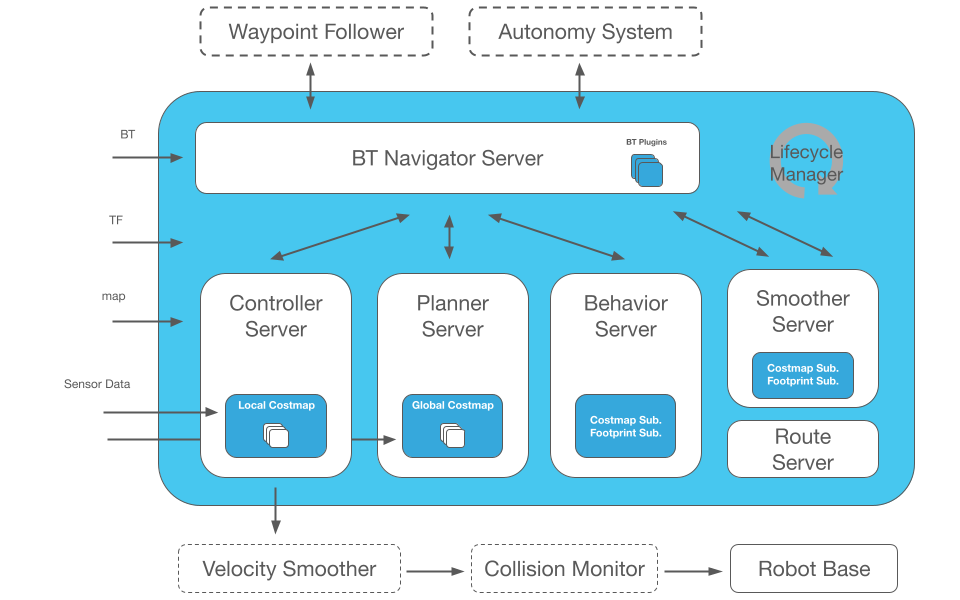
\includegraphics[width=14cm]{nav2_architecture}
\end{figure}

В Nav2 есть инструменты для:
\begin{itemize}
	\item загрузки, обслуживания и хранения карт;
	\item локализации робота по предоставленной карте (SLAM предоставляет начальную
		карту);
	\item планирования полного пути через окружающую среду;
	\item управления роботом, чтобы он следовал по маршруту и динамически
		корректировался, чтобы избежать столкновений;
	\item сглаживания маршрутов, чтобы сделать их более непрерывными, плавными
		и/или выполнимыми.
	\item преобразование данных датчиков в модель окружающего мира;
	\item построение сложных и настраиваемых моделей поведения роботов с
		помощью деревьев поведения;
	\item выполнение заранее определенных действий в случае сбоя, вмешательства
		человека или других ситуаций;
	\item выполнение последовательных маршрутных точек, составляющих миссию;
	\item управление жизненным циклом программы и сторожевым таймером для
		серверов;
	\item простые динамически загружаемые плагины для создания индивидуальных
		алгоритмов, поведений и т. д.
	\item мониторинг необработанных данных датчиков на предмет неминуемого
		столкновения или опасной ситуации;
\end{itemize}

\subsection{Анализ пакетов решающих задачу навигации, локализации и построения
карты}

Для навигации мобильной системы необходима карта, для построения которой
используют SLAM (Одновременную локализацию и построение карты). 

Алгоритмы SLAM можно разделить на две группы: более ранние алгоритмы,
использующие подходы, основанные на фильтрах Байеса , и более новые методы,
основанные на графах. Значимые реализации на основе фильтров, доступные в виде
пакетов \ros{} это: GMapping и HectorSLAM . Cartographer и KartoSLAM являются
основными доступными реализациями на основе графов \cite{macenski2021slam}.

Рассмотрим пакеты ros{}, такие как: SLAM Toolbox и GMapping:
\begin{itemize}
	\item SLAM Toolbox -- использует подход оптимизации
		графов.
	\item GMapping \cite{grisetti2005improving} -- использует Rao–Blackwellized
		Particle Filter (Фильтр частиц с использование теоремы Рао — Блэквелла —
		Колмогорова )
\end{itemize}


В SLAM Toolbox есть возможность делать почти всё, что есть в любой другой
платной и бесплатной библиотеке SLAM. Это включает в себя:
\begin{itemize}
	\item обычный точечный 2D SLAM для мобильных роботов (старт, карта,
		сохранение pgm-файла) с некоторыми хорошими встроенными утилитами,
		такими как сохранение карт;
	\item продолжение уточнения, перестройки карты или продолжения построения
		карты сохраненного (сериализованного) графа позиций в любое время;
	\item пожизненное картирование: загрузите сохраненный граф позиций и
		продолжайте строить карту, одновременно удаляя лишнюю
		информацию из новых сканов;
	\item режим локализации на основе оптимизации, построенный на основе
		pose-графа. Возможность запуска режима локализации без предварительной
		карты для режима «лидарной одометрии» с локальным замыканием контуров;
	\item синхронный и асинхронный режимы отображения;
	\item объединение кинематических карт (в разработке находится техника
		объединения манипуляций с эластичным графом);
	\item оптимизационные решатели на основе плагинов с новым оптимизированным
		плагином на основе Google Ceres;
	\item плагин RVIZ для взаимодействия с инструментами;
	\item инструменты манипулирования графами в RVIZ для манипулирования узлами
		и связями во время отображения;
	\item сериализация карт и хранение данных без потерь.
\end{itemize}

В то время как пакет GMapping предлагает обёртку над алгоритмом,
описанным в статье \cite{grisetti2005improving}, где предполагается построение и
сохранение карты, отстутствует.

\begin{figure}[h]
	\caption{Пример построения карты используя SLAM Toolbox (слева) и GMapping
	(справа).}
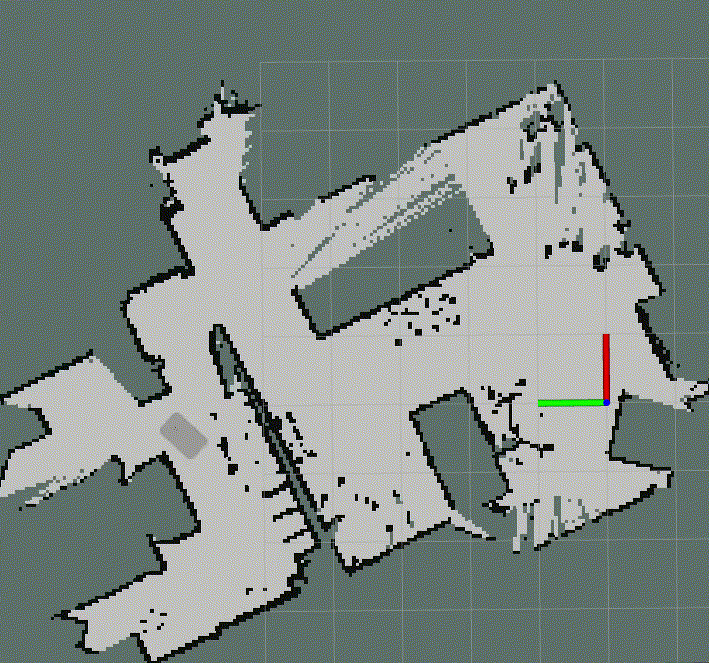
\includegraphics[width=7cm]{slam_toolbox_example}
\centering
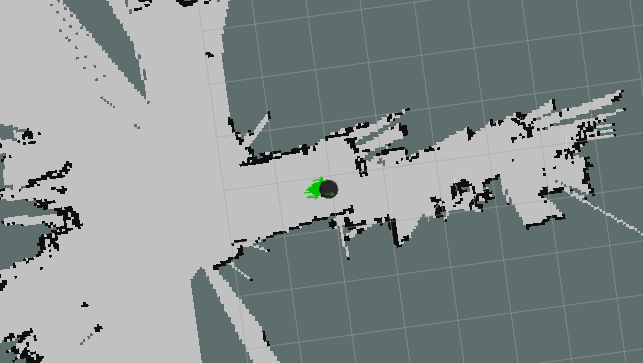
\includegraphics[width=7cm]{gmapping_example}
\end{figure}


%Но у этого архитектурного подхода есть ряд недостатков: дополнительные затраты
%на сериализацию и десериализацию данных, затраты на маршрутизацию сообщений. А
%также при использовании нескольких программных модулей, конечный программный
%продукт по своей сути является распределённой системой, включая все плюсы и
%минусы распределённых систем, такие как:
%
%\begin{itemize}
%	\item Проблемы с синхронизацией состояния, неконсистентность состояния.
%	\item Потеря сообщений.
%	\item Каскадный отказ системы.
%	\item Невозможность использования отладчика для отладки всей системы.
%\end{itemize}


% BIG SECTION
	\section{Моделирование предметной области и разработка функциональных требований}

\subsection{Формирование требований к проектируемому программному средству}
%%%%%%%%%%%%%

Для успешной реализации системы мобильной навигации необходимо четко определить
и описать функциональные требования, которые будут обеспечивать эффективность и
точность работы системы. Эти требования являются основой для проектирования и
разработки как аппаратной, так и программной части системы. В данном разделе мы
рассмотрим ключевые аспекты, которые должны быть учтены при разработке
функциональных требований для мобильной навигации, включая работу с картами,
выполнение маршрутов и интеграцию различных сенсоров.

Первым и основным требованием является способность системы точно определять свое
местоположение. Это должно включать в себя использование различных сенсоров,
таких как GPS, гироскопы, акселерометры и камеры, которые обеспечат точную
локализацию устройства как в открытых, так и в закрытых помещениях. Для этого
система должна использовать алгоритмы, обеспечивающие непрерывную и стабильную
локализацию в реальном времени, минимизируя погрешности и ошибки.

Важным аспектом является способность системы создавать карту окружающей среды на
основе данных от сенсоров. Для этого применяется технология SLAM (Simultaneous
Localization and Mapping), которая позволяет одновременно и локализовать
устройство, и строить карту его окружения. Эта карта должна быть динамической и
изменяться в зависимости от новых данных, полученных от сенсоров.

Для обеспечения точности навигации система должна эффективно обрабатывать данные
с различных сенсоров, таких как камеры, лидары, ультразвуковые датчики, и
объединять их в единую модель пространства. Обработка этих данных должна
происходить с минимальной задержкой, чтобы система могла адекватно реагировать
на изменения в окружающей среде и корректировать маршрут в реальном времени.

На основе карты окружающей среды и информации о текущем местоположении, система
должна быть способна планировать оптимальный маршрут до заданной цели.
Планирование маршрута должно учитывать не только расстояние, но и такие факторы,
как препятствия, зоны с ограничениями, а также предпочтения пользователя
(например, избегать оживленных улиц или труднопроходимых территорий).

После того как маршрут спланирован, система должна быть способна проводить
устройство по этому маршруту. Для этого требуется реализация алгоритмов, которые
будут учитывать динамичные изменения в окружении и корректировать маршрут в
случае появления новых препятствий или изменения дорожных условий. Система
должна предоставлять пользователю понятные и своевременные подсказки о следующем
шаге, а также информацию о текущем статусе маршрута.

Важно, чтобы система могла адаптироваться к изменениям окружающей среды, таким
как перемещающиеся объекты или изменения в инфраструктуре. Для этого система
должна использовать алгоритмы, способные перераспределять маршрут на лету,
минимизируя влияние изменений на навигацию и обеспечивая бесперебойное
выполнение маршрута.

Важным требованием является возможность интеграции системы с внешними
источниками данных, такими как онлайн-карты, базы данных о пробках,
актуальная информация о дорожной ситуации и погодных условиях. Это позволит
системе учитывать внешние факторы, влияющие на движение, и корректировать
маршрут с учетом текущей ситуации.

В результате правильной разработки и внедрения данных функциональных требований
можно создать систему, которая будет эффективно и точно выполнять задачи
мобильной навигации в различных условиях, предоставляя пользователю удобный и
безопасный опыт взаимодействия с устройством.

\begin{itemize}
	\item Отправка управляющих сигналов на мобильную платформу
	\item SLAM
	\item Оценка позиции робота
\end{itemize}

% BIG SECTION
	\section{Проектирование программного средства}

\subsection{Описание модулей системы}
Для реализации системы мобильной навигации были выбраны три ключевых датчика:
\begin{itemize}
	\item 2D Lidar;
	\item IMU;
	\item GPS.
\end{itemize}



Эти датчики обеспечивают систему данными о пространстве, в котором находится
робот, его ориентации и глобальном местоположении, что критически важно для
корректной работы алгоритмов локализации и построения маршрута.
2D Lidar позволяет получать информацию о препятствиях вокруг устройства, IMU
предоставляет данные о наклоне и угловых ускорениях, а GPS — о глобальной
позиции робота. Все эти данные интегрируются в систему навигации, создавая
основу для безопасного и эффективного перемещения устройства в различных
условиях.

2D Lidar (Light Detection and Ranging) работает на основе принципа измерения
расстояния до объектов с использованием лазерных импульсов. Ли дар излучает
лазерные импульсы, которые отражаются от объектов, встречающих их на пути.
Время, которое требуется импульсу для прохождения от лидара до объекта и
обратно, используется для вычисления расстояния до объекта. Этот процесс
повторяется многократно по всей области сканирования, создавая карту расстояний
на основе измерений.

\begin{figure}[h]
\caption{2D Lidar}
\centering
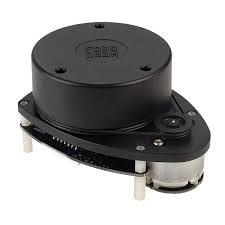
\includegraphics[width=9cm]{2d_lidar}
\end{figure}

2D лидары обычно работают в плоскости, что означает, что они измеряют расстояния
только в одном направлении (по горизонтали или вертикали). Сканер вращается или
перемещается по оси, чтобы покрыть широкую область, создавая двумерное
изображение окружающего пространства. С помощью таких данных система может
строить карту и распознавать объекты, определяя их положение и расстояние до
них, что крайне важно для навигации роботов и беспилотных автомобилей.

IMU (Inertial Measurement Unit) — это датчик, который измеряет и сообщает
информацию о движении и ориентации объекта в пространстве. Он состоит из трех
основных компонентов: акселерометров, гироскопов и иногда магнитометров.
Акселерометры измеряют ускорения по трем осям (X, Y, Z), что позволяет
определить изменение скорости и положение объекта относительно земной
гравитации. Гироскопы отслеживают угловые скорости вращения вокруг тех же осей,
что помогает измерять ориентацию объекта и его вращения. Магнитометры, если они
присутствуют, измеряют магнитное поле Земли, что позволяет дополнительно
корректировать ориентацию.

Принцип работы IMU заключается в интеграции данных с этих сенсоров, чтобы
получить полное представление о движении и положении объекта. Например,
акселерометры могут обнаружить, если устройство наклоняется или ускоряется, а
гироскопы отслеживают угловые изменения, такие как вращение вокруг своей оси.
Это позволяет системе вычислить изменения ориентации и траекторию движения, что
полезно в таких приложениях, как робототехника, авиация и навигация в условиях
отсутствия GPS.

GPS — это навигационная система, основанная на использовании спутников для
определения местоположения объектов на Земле. Система состоит из спутников,
находящихся на орбите, наземных станций и приемников, которые используются для
получения данных о местоположении. Спутники передают сигналы с точным временем,
и приемник на Земле, получая эти сигналы от нескольких спутников, может
вычислить свое местоположение.

Принцип работы GPS заключается в измерении времени, которое требуется сигналу,
чтобы добраться от спутника до приемника. Поскольку спутники известны своей
точной орбитой, приемник может определить расстояние до каждого спутника,
используя это время. Получая сигналы от как минимум четырех спутников, приемник
может точно вычислить свою абсолютную позицию в трехмерном пространстве —
определяя широту, долготу и высоту, а также время. Эти данные обеспечивают
высокую точность определения местоположения, что критически важно для навигации
и локализации в реальном времени.

Проектирование системы мобильной навигации начинается с разработки архитектуры
программного обеспечения, которая должна обеспечивать взаимодействие между
несколькими ключевыми модулями. Эти модули включают сбор данных с сенсоров,
алгоритм SLAM для построения карты и локализации робота, оценку текущего
положения, планирование маршрута и управление моторами. Каждый из этих
компонентов должен работать эффективно и в реальном времени, обеспечивая
точность и стабильность работы системы.

Первым этапом является сбор данных с сенсоров. 2D Lidar предоставляет информацию
о расстояниях до объектов в окружающем пространстве, IMU — данные об угловых
ускорениях и наклоне устройства, а GPS — информацию о глобальном местоположении.
Все эти данные передаются в алгоритм SLAM, который использует их для построения
карты окружающей среды и вычисления текущего местоположения робота. Это
позволяет системе иметь точную картину окружающего мира и следить за положением
устройства.

Алгоритм SLAM является основой для построения карты и локализации робота. С
помощью данных от лидаров и других сенсоров он строит карту пространства,
постоянно обновляя ее по мере движения робота, и вычисляет его местоположение
относительно этой карты. Это позволяет системе динамично корректировать действия
робота в зависимости от изменений в окружающей среде, таких как появление новых
препятствий или изменение положения объектов.

Полученные от SLAM данные о местоположении робота передаются в модуль оценки
позиции. Этот модуль анализирует текущее положение устройства с использованием
фильтрации и различных методов оценки, таких как фильтр Калмана. Оценка позиции
робота имеет важное значение для корректного планирования маршрута, поскольку
точность информации о местоположении напрямую влияет на точность движений
устройства.

Модуль проложения маршрута отвечает за вычисление оптимального пути от текущего
местоположения робота до заданной цели. Этот модуль использует данные о
местоположении, а также информацию о препятствиях, чтобы планировать наиболее
эффективный и безопасный маршрут. Важно, чтобы система могла адаптироваться к
изменениям окружающей среды, например, при возникновении новых препятствий,
система должна пересчитать маршрут в реальном времени, обеспечивая продолжение
движения робота без ошибок.

После того как маршрут спланирован, информация о нем передается в модуль
управления моторами. Этот модуль отвечает за выполнение команд, таких как
движение вперед, повороты и торможение. Модуль управления моторами должен
обеспечить точное выполнение команд с минимальными задержками, чтобы робот мог
двигаться по маршруту с высокой точностью. Кроме того, он должен поддерживать
оперативную реакцию на данные от сенсоров, такие как сигнал от лидаров,
предупреждающий о близко расположенных препятствиях.

При обнаружении препятствий вблизи, например, если расстояние до объекта
становится меньше заданного порога, система должна немедленно реагировать. Это
может быть реализовано командой «стоп», которая отправляется в модуль управления
моторами для немедленной остановки робота. Такие меры безопасности необходимы
для предотвращения столкновений и обеспечения безопасной работы робота в
различных условиях.

Важным аспектом проектирования является создание четко структурированных и
эффективных протоколов взаимодействия между модулями. Каждый компонент системы
должен обмениваться данными с другими через заранее определенные интерфейсы, что
позволит избежать конфликтов и обеспечит стабильную работу всей системы. Это
также упрощает тестирование и отладку, а также позволяет легко заменять или
обновлять отдельные компоненты системы без нарушения работы всей системы.

\subsection{Язык программирования}

Для реализации такой системы был выбран язык программирования Rust. Этот язык
был выбран благодаря его высоким характеристикам безопасности,
производительности и поддержке многозадачности. Rust обладает уникальной
системой владения и заимствования, которая предотвращает ошибки управления
памятью, такие как утечки памяти или доступ к уже освобожденным данным. Это
крайне важно для разработки критичных систем реального времени, таких как
мобильные роботы, где даже небольшие ошибки могут привести к сбоям в работе.

Одним из ключевых преимуществ Rust является его способность обеспечивать
безопасность многозадачности. В отличие от C++, который требует дополнительных
усилий для безопасного выполнения параллельных операций, Rust изначально
предусматривает механизмы предотвращения гонок данных, что делает код более
надежным. Это особенно важно для системы навигации, где необходимо параллельно
обрабатывать данные с различных сенсоров и вычислять управляющие команды без
риска возникновения ошибок синхронизации.

Rust также предоставляет встроенные инструменты для работы с асинхронным
программированием, что позволяет эффективно организовать обработку данных в
реальном времени. Асинхронные операции позволяют системе собирать данные с
сенсоров, планировать маршрут и управлять моторами без блокировки основного
потока выполнения, что способствует повышению производительности и снижению
задержек.

Программная экосистема Rust активно развивается, и существует множество
библиотек, которые могут быть использованы для решения задач, связанных с
обработкой сенсорных данных, математическими расчетами и оптимизацией маршрутов.
Это позволяет разработчикам легко интегрировать необходимые инструменты и
сокращать время на разработку и тестирование системы. Также, благодаря хорошей
поддержке со стороны сообщества, Rust предоставляет разработчикам множество
ресурсов для быстрого решения возникающих вопросов.

Ключевым преимуществом Rust является его кроссплатформенность. Код, написанный
на этом языке, может быть скомпилирован для различных платформ, что делает Rust
отличным выбором для мобильных роботов, которые могут работать на разных типах
оборудования. Это позволяет без значительных усилий адаптировать систему под
разные архитектуры и аппаратные платформы.

Будущие улучшения системы могут включать в себя добавление новых сенсоров,
улучшение алгоритмов SLAM и маршрутизации, а также интеграцию с внешними
системами, такими как онлайн-карты или системы для прогнозирования дорожной
ситуации. Rust, благодаря своей гибкости и безопасному управлению памятью,
идеально подходит для такой работы, обеспечивая долгосрочную устойчивость и
развитие проекта.

Таким образом, проектирование программного обеспечения для системы мобильной
навигации с использованием сенсоров и алгоритмов SLAM требует тщательной
проработки архитектуры, выбора эффективных технологий и инструментов. Язык Rust
является отличным выбором для разработки таких систем, благодаря своим
преимуществам в безопасности, производительности и поддержке многозадачности,
что делает его идеальным для создания высоконадежных и высокопроизводительных
приложений для робототехники.



\setcounter{section}{6}
% BIG SECTION
% CUTOFF
	%\section{Разработка программного средства}
	%\section{Тестирование работоспособности программного средства}
	\section[7]{Технико-экономическое обоснование разработки и использования
	программного средства навигации мобильных систем}

\subsection{Характеристика программного средства}
Программное средство навигации мобильных систем осуществляет задачу перемещения
и определения местоположения мобильной системы, построение и исполнение 
маршрута с использованием сенсоров и приводов. \appname{} оптимизировано для
навигации голономных колёсных роботов. Предполагается что мобильная система 
управляется через отправку команды установки угловой и линейной скорости. 
Также необходима конфигурация под размеры и движение каждого определённого
робота.

\appname{} выполняет следующие функции:

\begin{itemize}
	\item сбор данных с датчиков;
	\item расчёт текущей позиции;
	\item построение карты;
	\item сохранение и загрузка карты;
	\item планирование маршрута;
	\item планирование движения;
	\item исполнение маршрута, учитывая динамические препятствия.
\end{itemize}


В сравнении с \ros{}, который является наиболее популярным аналогом, \appname{}
упрощает развёртывание, требует меньше вычислительных ресурсов за счёт
минимизации затрат на общении модулей путём расположения их в одном процессе
операционной системы, что позволяет использовать менее мощное аппаратное
обеспечение.

\appname{} получает данные с датчиков, информацию о цели которой ей 
необходимо достигнуть  и отправляет управляющие сигналы на ходовую часть. 
Решается задача локализации, построения маршрута и выполнения маршрута 
к заданной точке. 

\subsection{Расчёты затрат на разработку программного средства}

Расчет затрат на разработку ПО производится в разрезе следующих статей затрат:

\begin{itemize}
	\item затраты на основную заработную плату разработчиков;
	\item затраты на дополнительную заработную плату разработчиков;
	\item отчисления на социальные службы;
	\item прочие затраты (амортизационные отчисления, расходы на 
		электроэнергию, командировочные расходы, арендная плата за офисные
		помещения и оборудование, расходы на управление и реализацию и т. п.).
\end{itemize}

Расчёт основной заработной платы осуществляется по формуле

\begin{equation}
	\label{eq:зарплата}
	\text{З}_o = \text{К}_{\text{пр}}\sum_{i=0}^{n} \text{З}_{\text{ч}i} \cdot t_i
	\ \text{,}
\end{equation}


\begin{explanationx}
	\item[где]  $n$  -- категории исполнителей, занятых разработкой
		программного средства;
	\item $\text{К}_\text{пр}$ - коэффициент премий и иных стимулирующих
		выплат (\num{1.3});
	\item $\text{З}_\text{ч}$ --  Часовой оклад исполнителя $i\text{-й}$
		категории, р.;
	\item $t$  -- трудоёмкость работ, выполняемых исполнителем $i\text{-й}$
		категории, ч.
\end{explanationx}


\subsubsection{} Затраты на основную заработную плату команды разработчиков
делятся исходя из численности, состава команды (категорий исполнителей), 
размеров месячной заработной платы каждого из участников команды, а также
общей трудоёмкости разработки ПО. 

\def \hoursPerMonth {167}

Согласно постановлению Министерства труда и социальной защиты Республики
Беларусь от 15 ноября 2024 г. \No 67 «Об установлении расчетной нормы рабочего
времени на 2024 год» при полной норме продолжительности рабочего времени на
2025 год для пятидневной рабочей недели с выходными днями в субботу и
воскресенье расчетная норма рабочего времени составит \num{2007} ч. На основании
этих данных среднее количество рабочих ч. в месяце принято равным
\hoursPerMonth{} ч.

Трудоёмкость определялась на основе сложности разработки программного средства,
объема функций. За основу в том числе брались фактические значения трудоёмкости
работ при разработке ПО со схожим функционалом в месте прохождения 
преддипломной практики.

Для расчёта возьмём размер премии 20\%.

На основании плановых данных был выполнен расчет основной заработной платы
команды разработчиков, результаты которого приведены в таблице~\ref{table:initialCost}.

\def \devSalary {2700}
\def \devAmountOfHours {458}
\FPeval{\devHourlySalary}{round(\devSalary / \hoursPerMonth, 2)}
\FPeval{\devCost}{round(\devAmountOfHours * \devHourlySalary, 2)}

\def \testSalary {2100}
\def \testAmountOfHours {200}
\FPeval{\testHourlySalary}{round(\testSalary / \hoursPerMonth, 2)}
\FPeval{\testCost}{round(\testAmountOfHours * \testHourlySalary, 2)}

\def \managerSalary {2500}
\def \managerAmountOfHours {120}
\FPeval{\managerHourlySalary}{round(\managerSalary / \hoursPerMonth, 2)}
\FPeval{\managerCost}{round(\managerAmountOfHours * \managerHourlySalary, 2)}

\FPeval{\costSum}{round(\devCost + \testCost + \managerCost, 2)}
\FPeval{\costBonuses}{round(\costSum * 0.2, 2)}
\FPeval{\costTotal}{round(\costSum + \costBonuses, 2)}

% МетУказ ТЭО ДП 2025
% Если в столбце таблицы у всех значений отсутствует дробная часть,
% дописывать нули после запятой не надо.

%\FloatBarrier
%\bgroup
%\def\arraystretch{1.7}
\nohyphens{
	\begin{longtable}{| p{3.5cm} | p{3.5cm} | l | l | l | r |}
		\caption{Расчёт основной заработной платы команды разработчиков}
		\label{table:initialCost} \\
		\hline 
		Наименование должности разработчика
		& Вид выполненной работы
		%& \raisebox{-2cm}{\rotatedtext{\parbox{3.5cm}
		%	{\centering Вид выполненной работы}}}
		& \raisebox{-2cm}{\rotatedtext{\parbox{3.5cm}
			{\centering Месячная заработная плата, р.}}}
		& \raisebox{-2cm}{\rotatedtext{\parbox{3.5cm}
			{\centering Часовая заработная плата, р.}}}
		& \raisebox{-2cm}{\rotatedtext{\parbox{3.5cm}
			{\centering Трудоёмкость работ, ч}}}
		& \raisebox{-2cm}{\rotatedtext{\parbox{3.5cm}
			{\centering Сумма, р.}}}
		\\ \hline 
		\endfirsthead

		Руководитель проекта
		& Координация работы, контроль сроков и этапов разработки
		& \num{\managerSalary}
		& \num{\managerHourlySalary}
		& \num{\managerAmountOfHours}
		& \num{\managerCost}
		\\ \hline 

		Инженер-программист 
		& Разработка программного средства  
		& \num{\devSalary}
		& \num{\devHourlySalary}
		& \num{\devAmountOfHours}
		& \num{\devCost}
		\\ \hline 

		Специалист по тестированию программного обеспечения
		& Тестирование программного средства
		& \num{\testSalary}
		& \num{\testHourlySalary}
		& \num{\testAmountOfHours}
		& \num{\testCost}
		\\ \hline 

		\multicolumn{5}{|l|}{Итого}
		& \num{\costSum}
		\\ \hline

		\multicolumn{5}{|l|}{Премия (20\%)}
		& \num{\costBonuses}
		\\ \hline

		\multicolumn{5}{|l|}{Общая сумма затрат на разработку}
		& \num{\costTotal}
		\\ \hline
	\end{longtable}
}
%\end{table}
%\egroup
%\FloatBarrier

\subsubsection{}
Расчёт затрат на дополнительную заработную плату команды разработчиков.

Затраты на дополнительную заработную плату команды разработчиков включают
выплаты, предусмотренные законодательство о труде (оплата трудовых отпусков,
льготных ч., времени выполнения государственных обязанностей и других выплат,
не связанных с основной деятельностью исполнителей), и определяются по формуле

\begin{equation}
	\text{З}_\text{д} = \frac{\text{З}_\text{о} \cdot
	\text{Н}_\text{д}}{\num{100}}
	\ \text{,}
\end{equation}

\begin{explanationx}
	\item[где] $\text{З}_\text{о}$ -- затраты на основную заработную плату;
	\item $\text{Н}_\text{д}$ -- норматив дополнительной заработной платы
		(\num{15}\%).
\end{explanationx}

Дополнительная заработная плата составит

\FPeval{\additionalSalary}{round(\costTotal * 0.15, 2)}

\begin{equation}
	\text{З}_\text{о} = \frac{\num{\costTotal} \cdot \num{15}}{\num{100}} =
	\num{\additionalSalary}
	\ \text{р.}
\end{equation}


Отчисления на социальные нужды определяются по формуле

\begin{equation}
	\text{Р}_\text{соц} = \frac{(\text{З}_\text{о} + \text{З}_\text{д}) \cdot
	\text{Н}_\text{соц}}{\num{100}}
	\ \text{,}
\end{equation}

\begin{explanationx}
	\item[где] $\text{Н}_\text{соц}$ -- норматив отчислений от фонда оплаты
		труда (35\%).
\end{explanationx}

Отчисления на социальные нужды составят

\FPeval{\socialCost}{round((\costTotal + \additionalSalary) * 0.35, 2)}
\begin{equation}
	\text{Р}_\text{соц} = \frac{(\num{\costTotal} + \num{\additionalSalary}) \cdot
	\num{35}}{\num{100}} = \num{\socialCost}
	\ \text{р.}
\end{equation}

Прочие затраты рассчитываются по формуле

\begin{equation}
	\text{Р}_\text{пз} = \frac{\text{З}_\text{о} \cdot \text{Н}_\text{пз}}{\num{100}}
	\ \text{,}
\end{equation}

\begin{explanationx}
\item[где] $\text{Н}_\text{пз}$ -- норматив прочих затрат, 35\%.
\end{explanationx}

Прочие затраты составят

\FPeval{\etcCost}{round(\costTotal * 0.35, 2)}
\begin{equation}
	\text{Р}_\text{пз} = \frac{\num{\costTotal} \cdot \num{35}}{\num{100}} = \num{\etcCost}
	\ \text{р.}
\end{equation}

Общая сумма затрат на разработку рассчитывается по формуле
\begin{equation}
	\text{З}_\text{общ} = 
	\text{З}_\text{о} +
	\text{З}_\text{д} +
	\text{Р}_\text{соц} +
	\text{Р}_\text{пз}
	\ \text{.}
\end{equation}

\FPeval{\finalCost}{round(\costTotal + \additionalSalary + \socialCost +
\etcCost, 2)}

Расчёт затрат на разработку программного продукта предоставлен в таблице~\ref{table:totalCost}

\FloatBarrier
\begin{table}
	\caption{Затраты на разработку программного обеспечения}
	\label{table:totalCost}
	\begin{tabular}{|l|r|}
		\hline
		Наименование статьи затрат
		& Значение, р.
		\\ \hline

		1. Основная заработная плата разработчиков
		& \num{\costTotal}
		\\ \hline

		2. Дополнительная заработная плата разработчиков
		& \num{\additionalSalary}
		\\ \hline

		3. Отчисления на социальные нужды
		& \num{\socialCost}
		\\ \hline

		4. Прочие затраты
		& \num{\etcCost}
		\\ \hline

		Общая сумма инвестиций в разработку
		& \num{\finalCost}
		\\ \hline
	\end{tabular}
\end{table}
\FloatBarrier

\subsection{Экономический эффект от разработки программного обеспечения и
применения программного обеспечения для собственных нужд}

В общем виде экономический эффект при использовании ПО рассчитывается по формуле
по формуле
\begin{equation}
	\Delta\text{П}_\text{ч} = (\text{Э}_\text{з} - \text{И}_\text{разр} -\Delta\text{З}_\text{тек})
	\cdot (1 - \frac{\text{Н}_\text{п}}{\num{100}})
	\ \text{,}
\end{equation}

\def \nalogNaPribil{20}

\begin{explanationx}
	\item[где] $\text{Э}_\text{з}$ -- экономия текущих затрат, полученная в
		результате применения ПО, р.;
	\item $\text{И}_\text{разр}$ -- затраты на разработку программного
		обеспечения, р.
	\item $\Delta\text{З}_\text{тек}$ -- прирост текущих затрат, связанных с
		поддержкой и сопровождением ПО, р.;
	\item $\text{Н}_\text{п}$ -- ставка налога на прибыль согласно действующему
	законодательству (\nalogNaPribil\%).
\end{explanationx}

% Дополнительная стоимость для сопровождения, в процентах
\def \additionalSupportCost {10}
\FPeval{\supportCost}{round(\finalCost * \additionalSupportCost / 100, 2)}
Прирост текущих затрат, связанных с сопровождением и поддержкой ПО, примем за
\num{\additionalSupportCost}\% от затрат на разработку ПО, что составит
\begin{equation}
	\text{З}_\text{тек} = \num{\finalCost} \cdot
	\frac{\num{\additionalSupportCost}}{\num{100}} = \num{\supportCost}
	\ \text{р.}
\end{equation}

% TODO, использование заменить на применение, но это уже было согласовано и абобус

Использование данного программного средства позволяет использовать более дешёвое
аппаратное обеспечение. Так как навигация и SLAM являются ресурсоёмкими
операциями, обычно используют компьютер \linebreak{} \hfill{}
NVIDIA~Jetson~Nano, стоимостью \num{1421.83} р.,
в то время как \appname{} позволяет использовать
Banana~Pi~CM4, стоимостью \num{300.12} р.

\FPeval{\savingsResult}{round(1421.83 - 300.12, 2)}
\def \robotCount {40}
\FPeval{\costWin}{round(\robotCount * \savingsResult, 2)}

Это позволяет экономить \num{\savingsResult} р. на единицу продукции.
Если взять в расчёт что в год производится  \num{\robotCount} мобильных систем,
получаем экономию текущих затрат в \num{\costWin} р.

\FPeval{\totalWin}{round((\costWin - \supportCost - \finalCost) * (1 -
0.\nalogNaPribil), 2)}

Экономический эффект для организации-заказчика при использовании ПО и выпуске
партии в \num{\robotCount} единиц составляет
\begin{equation}
	\Delta\text{П}_\text{ч} = (\num{\costWin} - \num{\finalCost} - \num{\supportCost}) \cdot
	(\num{1} - \frac{\num{\nalogNaPribil}}{\num{100}}) = \num{\totalWin}
	\ \text{р.}
\end{equation}

Уровень рентабельность затрат рассчитывается по формуле
\begin{equation}
	\text{У}_\text{р} = \frac{\Delta\text{П}_\text{ч}}{\text{И}_\text{разр}}
\cdot \num{100}
	\ \text{,}
\end{equation}

уровень рентабельности составляет

\FPeval{\rentabelnost}{round(\totalWin / \finalCost * 100, 2)}
\begin{equation}
	\text{У}_\text{р} = \frac{\num{\totalWin}}{\num{\finalCost}} \cdot \num{100}
	= \num{\rentabelnost}\%
	\ \text{.}
\end{equation}


\def \stavkaBankov {0.1376}

В результате расчёта были получены следующие показатели (см.~табл.~
\bgroup
\def\arraystretch{1.2}
\ref{table:hehelastone})
	\begin{longtable}{|p{10cm}|c|}
		\caption{Экономические показатели}  \label{table:hehelastone} \\
		\hline
		Наименование показателя
		& Значение
		\\ \hline

		Прогнозируемая сумма затрат на разработку программного продукта
		& \num{\finalCost}~р.
		\\ \hline

		Прирост чистой прибыли
		& \num{\totalWin}~р.
		\\ \hline

		Рентабельность инвестиций
		& \num{\rentabelnost}\%
		\\ \hline
	\end{longtable}
\egroup



Средняя процентная ставка по банковским депозитным вкладам на январь
2025-го г. не превышает \num{13.76}\% \cite{nbrb2025}, рентабельность инвестиций
в проект составляет \num{\rentabelnost}\%. Инвестиции в разработку проекта
окупятся за первый год реализации проекта. Это означает, что данный проект
программного средства навигации мобильных систем является экономический
эффективным, разработка и последующая продажа программного продукта являются
экономически целесообразными.


\renewcommand{\bibsection}{\sectioncentered*{Список использованной литературы}}
\bibliography{test}
\end{document}
